\chapter{Конструкторский раздел}

\vspace{-0.5cm}\hspace{0.6cm}В данном разделе будут рассмотрены типы и структуры данных, необходимые для решения поставленных задач. Будут формализованы алгоритм изменения положения точек полотна флага и алгоритм Z-буфера, а также будут описаны процесс рендера в целом и работа с камерой.

\section{Алгоритм изменения положения точек}
Формально последовательность действий в данном алгоритме можно описать следующим образом:

\begin{enumerate} 
	\item Определить вектора силы воздействия ветра.
	\begin{enumerate} 
		\item Для каждой грани:
		\begin{enumerate} 
			\item Определить вектор нормали.
			\item Определить угол между вектором нормали и вектором ветра.
			\item Задать вектор воздействия ветра на грань (значение вектор ветра, направление в соответствии с углом).
			\item Для каждой точки грани прибавить к результирующему векторы силы полученный вектор воздействия ветра.
		\end{enumerate}
	\end{enumerate}
	\item Определить вектора сил упругости и трения пружины.
	\begin{enumerate} 
		\item Для каждой «пружины»:
		\begin{enumerate} 
			\item Определить текущую длину пружину.
			\item Определить вектор силы трения как вектор, пропорциональный относительной скорости двух точек.
			\item Для каждой из двух вершин:
			\begin{enumerate}
				\item Определить вектор силы упругости.
				\item Прибавить к вектору силы трения.
				\item Прибавить к результирующему вектору силы суммарный вектор.
			\end{enumerate}
		\end{enumerate}
	\end{enumerate}
	\item Для каждой точки:
	\begin{enumerate}
		\item Определить вектор силы гравитации.
		\item Прибавить вектор силы гравитации к результирующему.
		\item Определить вектор силы трения.
		\item Прибавить данный вектор к результирующему.
		\item Найти ускорение точки путём интегрирования.
		\item Найти новую скорость.
		\item Изменить координаты точки в соответствии с найденной скоростью.
	\end{enumerate}
\end{enumerate}

Схемы данного алгоритма представлены на рис. \ref{fig:pos_overall}, рис. \ref{fig:pos_wind}, рис. \ref{fig:pos_spring}.

\pagebreak

\begin{figure}[ht!]
	\begin{center}
		\begin{minipage}[h]{0.4\linewidth}
			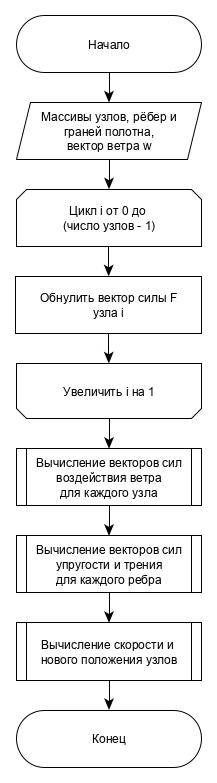
\includegraphics[scale=0.65]{pos_overall.jpg}
			\caption{Схема алгоритма вычисления нового положения точек}
			\label{fig:pos_overall}
		\end{minipage}
		\hfill 
		\begin{minipage}[h]{0.4\linewidth}
			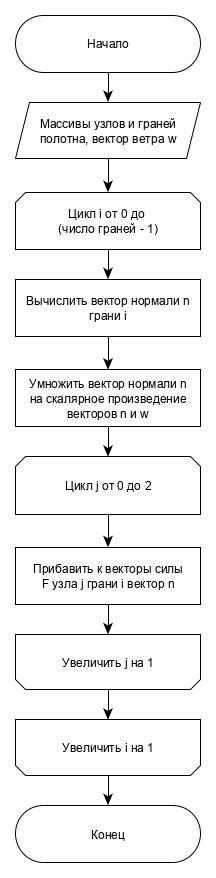
\includegraphics[scale=0.65]{pos_wind.jpg}
			\caption{Схема алгоритма вычисления векторов сил воздействия ветра}
			\label{fig:pos_wind}
		\end{minipage}
	\end{center}
\end{figure}

\begin{figure}[ht!]
	\centering
	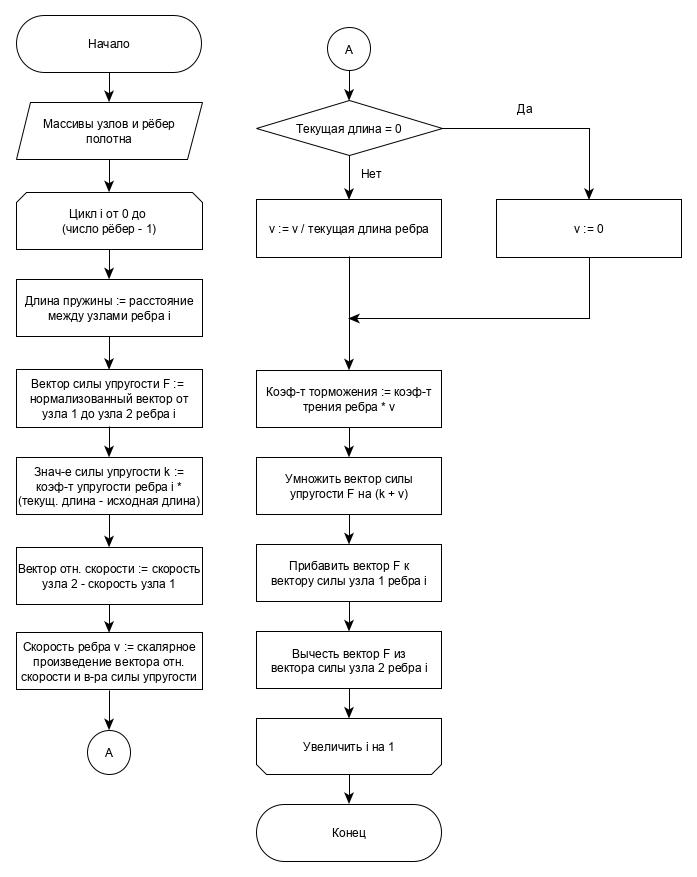
\includegraphics[scale=0.65]{pos_spring.jpg}
	\caption{Схема алгоритма вычисления векторов сил упругости и трения рёбер}
	\label{fig:pos_spring}
\end{figure}

\pagebreak

\section{Трёхмерные аффинные преобразования координат}
\hspace{0.6cm}В процессе работы программе возникает необходимость преобразования объектов сцены - их сдвига, масштабирования и поворота. Для трёхмерного пространства любо аффинное преобразование может быть представлено последовательностью простейших операций.

\vspace{0.2cm}Ниже приведены уравнения преобразований координат $(x, y, z)$ точки: 
\begin{itemize}
	\item сдвиг на $(dx, dy, dz)$:
		\begin{equation}
		\begin{cases}
		x_{new} = x + dx\\
		y_{new} = y + dy\\
		z_{new} = z + dz
		\end{cases}
		\label{eq:shift}
		\end{equation}
	\item масштабирование с коэффициентами $k_x, k_y, k_z$ относительно точки $C$
		\begin{equation}
		\begin{cases}
		x_{new} = x_C + k_x (x - x_C)\\
		y_{new} = y_C + k_y (y - y_C)\\
		z_{new} = z_C + k_z (z - z_C)
		\end{cases}
		\label{eq:scale}
		\end{equation}
	\item поворот на угол $\phi$ относительно
	\begin{itemize}
		\item оси X
			\begin{equation}
			\begin{cases}
			x_{new} = x\\
			y_{new} = y \cdot cos\phi - z \cdot sin\phi\\
			z_{new} = y \cdot sin\phi + z \cdot cos\phi\\
			\end{cases}
			\label{eq:rotx}
			\end{equation}
		\item оси Y
			\begin{equation}
			\begin{cases}
			x_{new} = z \cdot sin\phi + x \cdot cos\phi\\
			y_{new} = y\\
			z_{new} = z \cdot cos\phi - x \cdot cos\phi\\
			\end{cases}
			\label{eq:roty}
			\end{equation}
		\item оси Z
			\begin{equation}
			\begin{cases}
			x_{new} = x \cdot cos\phi - y \cdot sin\phi\\
			y_{new} = x \cdot sin\phi + y \cdot cos\phi\\
			z_{new} = z
			\end{cases}
			\label{eq:rotz}
			\end{equation}
	\end{itemize}
\end{itemize}

\section{Процесс отрисовки изображения}
\hspace{0.6cm}В качестве алгоритма визуализации объекта был выбран алгоритм Z-буфера. Формальное описание алгоритма Z-буфера:
\begin{enumerate}
	\item инициализировать и заполнить буфер кадра фоновым значением цвета;
	\item инициализировать и заполнить Z-буфер максимальным значением $z$;
	\item преобразовать каждый многоугольник в растровую форму в произвольном порядке; 
	\item для каждого пикселя в многоугольнике вычислить его глубину $z(x, y)$ или расстояние по оси $z$;
	\item сравнить глубину $z(x, y)$ со значением в Z-буфере в позиции $[x, y]$;
	\item если $z(x, y)$ > Z-буфер$(x, y)$, то записать атрибут (цвет, интенсивность и т. п.) в буфер кадра и в Z-буфер записать $z(x, y)$, иначе никаких действий не производить.
\end{enumerate}

На рис. \ref{fig:zbufferflow} представлен полный процесс отрисовки изображения.

\begin{figure}[ht!]
	\centering
	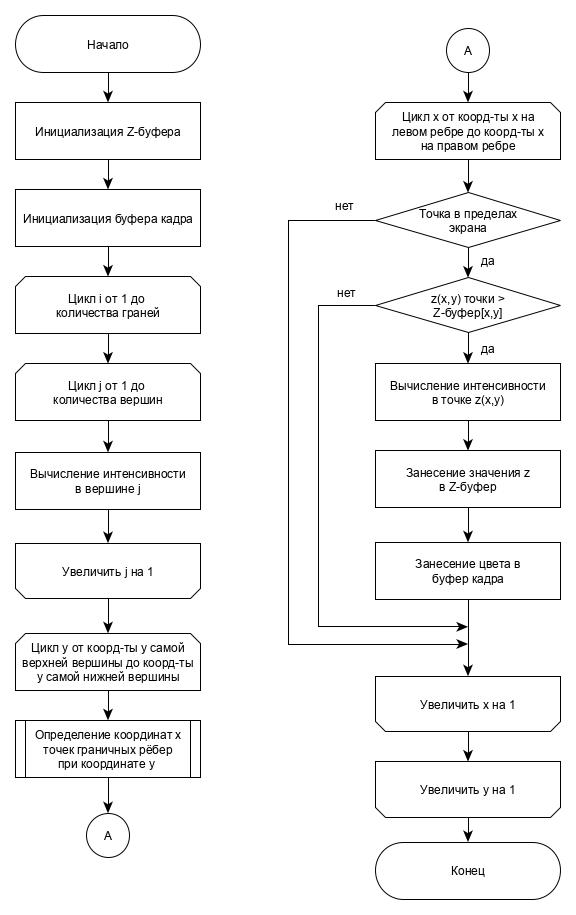
\includegraphics[scale=0.65]{zbuffer_scheme.jpg}
	\caption{Схема работы алгоритма Z-буфера}
	\label{fig:zbufferflow}
\end{figure}

\pagebreak

\section{Анимация объектов}
\hspace{0.6cm}Для моделирования развевающегося флага был выбран метод анимации по ключевым кадрам. В данном методе происходит изменение положения различных частей объекта от начального состояния до конечного. Плавность анимации осуществляется за счет просчитывания промежуточных состояний объекта. В данном случае своё положение меняют точки полотна флага в соответствии с системой уравнений \ref{eq:sys}. Каждый раз объект переходит из одного промежуточного состояния в другое и так, пока не достигнет конечного.

\section{Используемые типы и структуры данных}
\hspace{0.6cm}Для того, что было возможно задать объекты, необходимо ввести следующие структуры:
\begin{itemize}
	\item \textbf{вершина}: содержит координаты x, y, z;
	\item \textbf{грань (треугольник)}: содержит поля
	\begin{itemize}
		\item массив из индексов трёх вершин;
		\item цвет;
	\end{itemize}
	\item \textbf{модель}: содержит поля
	\begin{itemize}
		\item список <<вершин>>;
		\item список <<граней>> (<<треугольников>>).
	\end{itemize}
\end{itemize}

\vspace{0.2cm}Для работы алгоритма изменения положения точек полотна флага используются различные физические параметры. В связи с этим требуется ввести дополнительные структуры для точек полотна:
\begin{itemize}
	\item \textbf{узел}: содержит поля
	\begin{itemize}
		\item указатель на структуру <<вершина>>, к которому привязан узел;
		\item индекс данной вершины;
		\item начальное положение узла - структура <<вершина>>;
		\item значение массы узла и обратное значение массы (для упрощения вычислений);
		\item значение коэффициента трения в узле;
		\item математический вектор силы F;
		\item математический вектор силы v;
	\end{itemize}
	\item \textbf{ребро} (соединяет узлы): содержит поля
	\begin{itemize}
		\item индексы <<вершин>> двух <<узлов>>, которые <<ребро>> связывает;
		\item длина ребра в состоянии покоя (начальная длина);
		\item текущая длина ребра;
		\item значение коэффициента упругости ребра;
		\item значение коэффициента трения на ребре;
	\end{itemize}
	\item \textbf{флаг}: содержит поля
	\begin{itemize}
		\item структура <<модель>>, описывающая текущее состояние полотна флага;
		\item список <<узлов>> в текущем положении;
		\item список <<рёбер>> в текущем положении;
		\item структура <<модель>>, описывающая начальное состояние полотна флага;
		\item список <<узлов>> в начальном положении;
		\item список <<рёбер>> в начальном положении.
	\end{itemize}
\end{itemize}

\vspace{0.2cm}Для хранения объектов сцены в программе используется список структур <<модель>>. Все значения координат, физических параметров и прочих полей, требуемых при вычислении, описываются вещественным типом \textit{double} для получения более точных результатов при вычислении положения точек. Все индексы описываются целым типом \textit{int}.

\vspace{0.2cm}При рендере моделей значения координат округляются до целого для занесения в буфер кадра, так как пиксели неделимы. Также для выполнения математических действий, связанных с использованием математического вектора (сложения физических сил, вычисления интенсивности в точке), вводится соответствующая структура, которая
\begin{itemize}
	\item содержит в качестве полей свои координаты x, y, z;
	\item предусматривает операции
	\begin{itemize}
		\item определения длины вектора;
		\item сложения и вычитания векторов;
		\item умножения вектора на число;
		\item скалярного произведения векторов;
		\item векторного произведения векторов;
		\item нормализации вектора.
	\end{itemize}
\end{itemize}

\section{Вывод}
\hspace{0.6cm}В данном разделе было дано формальное описание алгоритмам нахождения нового положения точек полотна флага, отрисовки изображения (алгоритм Z-буфера), были приведены математические формулы, описывающие аффинные преобразования координат точек. Также были перечислены и описаны основные типы и структуры данных, использующиеся в проекте.
